\begin{itemize}
\item	N-Teir Architecture Diagram
\item	i.e. data flow diagram between the interface/client, middle ware, and backend services/data repos
\item	Describe the data model i.e. what data needs to be stored or persisted by the application?
\item	What are the relationships within the data model.
\item	i.e. use ER diagram and explain.
\item	Describe the backend services used (if any).
\item	Reflective Questions: 
\item	How have you ensured that there is a separation of concerns? 
\item	What other technology could have been used instead of django? 
\item	What are the advantages of using a Web Application Framework over other technology? 
\item	And, what are the disadvantages?
\end{itemize}


We used the N-tier diagram shown in figure \ref{fig:n-tier} which
shows the client (Web Browser), middleware (Django), the database and
the external service (Youtube API), to design our architecture.

\begin{figure}[h]
  \begin{center}
    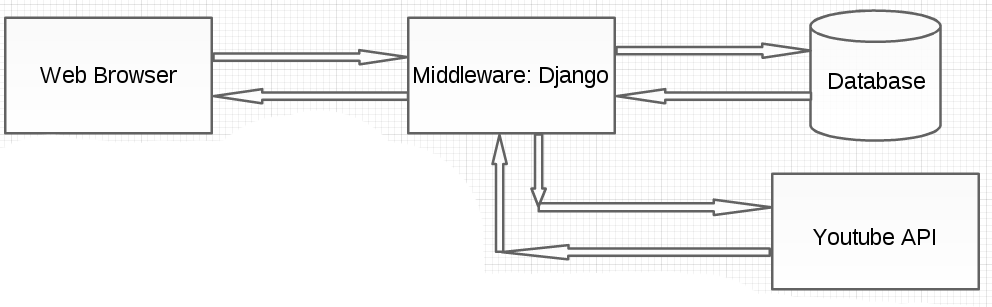
\includegraphics[width=0.45\textwidth]{ntier}
    \caption{N-Tier Diagram} \label{fig:n-tier}
  \end{center}
\end{figure}

As can be inferred from the diagram, the clients sends requests for
data to the middleware, this then retrieves the appropriate data from
the database or the external services as required and the data is sent
back through the middleware to the client.

Typically a request follows a structure similar to the following:
the client makes a request for a web page; the middleware retrieves
this request via specified url patterns which call particular view
methods for the app; this view will then make calls to the database to
retrieve appropriate data; the data will be taken by the view and then
passed back to the web browser via a http response according to the
template associated with the view; the client receives this and
displays the information.

In order to design the data models for our application we created an
Entity-Relationship diagram based on Chen notation
\cite{ChenNotation}.
This has been reconstructed and can be seen in figure \ref{fig:ER}.

\begin{figure}[h]
  \begin{center}
    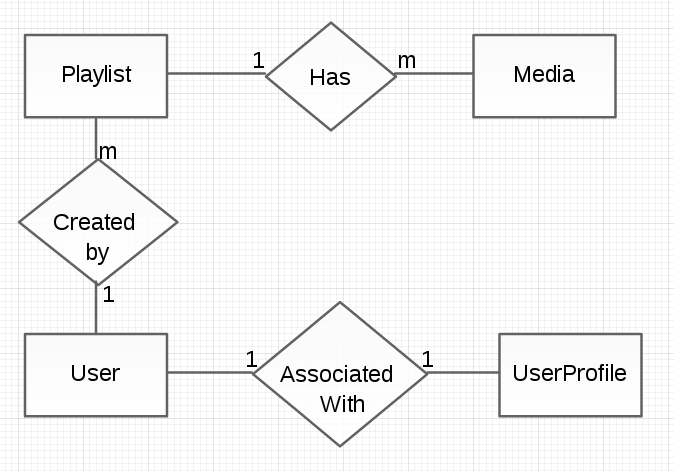
\includegraphics[width=0.45\textwidth]{ER}
    \caption{Entity-Relationship Diagram} \label{fig:ER}
  \end{center}
\end{figure}

\begin{itemize}
\item{Playlist}
  \begin{itemize}
  \item{Title: name of this playlist}
  \item{Creator: reference to the User who created this playlist}
  \item{Views: a count of the number of times this playlist has
      been viewed}
  \item{Url: the title of this playlist encoded for use in a url}
  \end{itemize}
\item{Media}
  \begin{itemize}
  \item{Playlist: reference to the playlist this media is associated
      with}
  \item{Name: name of this media}
  \item{Url: source url of this media}
  \item{Source: the domain of this media eg. YouTube}
  \item{Thumbnail: thumbnail image to be used for this media}
  \end{itemize}
\item{User}
  \begin{itemize}
  \item{(default User model from Django, the following fields are the
      specific fields taken from this model)}
  \item{Username}
  \item{Password}
  \item{Email}
  \end{itemize}
\item{UserProfile}
  \begin{itemize}
  \item{User: reference to User assosciated with this UserProfile}
  \item{Picture: image to be used as a profile picture}
  \end{itemize}
\end{itemize}

A key design element in consideration from the start of development
was separation of concerns.
Using many technologies (Django, Python, JavaScript, HTML, CSS etc.)
it was paramount that each of these be kept as seperate as possible so
that the source could remain readable.